\section{Experimental Results}\label{sec:benchmarks}

\subsection{Goals}

BigchainDB's algorithms are designed to ``get out of the way'' of the underlying database, so we expect the main limiter on performance to be how that underlying database interacts with the physical compute resources (e.g.~write speed and I/O among nodes).
Because of that, and because BigchainDB is built on top of RethinkDB, we began with experiments to test the scalability properties of RethinkDB.

Full benchmarks on the performance of BigchainDB will appear in the near future.

\subsection{Experiments on Throughput}

Appendix~\ref{subsec:benchmarks_setup} describes the details of the experimental setups.

In one experiment, we increased the number of nodes every ten seconds, up to $32$ nodes.
We used RethinkDB's System Statistics Table to record the write throughput over time.

\begin{figure}[!ht]
  \centering
  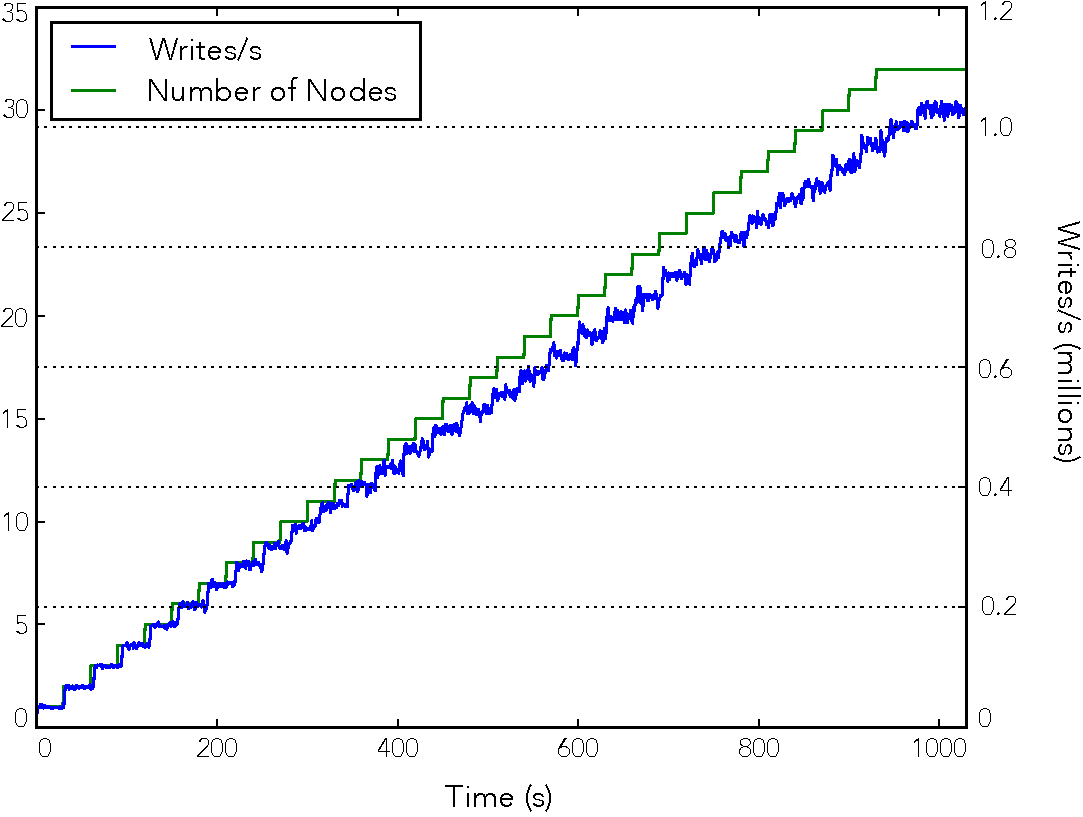
\includegraphics[width=0.7\textwidth]{figure_14.pdf}
  \caption{Time-series plot, where when we increased the number of nodes, the throughput increased proportionately.}
  \label{fig:bigchain_throughput_vs_nodes}
\end{figure}

Figure~\ref{fig:bigchain_throughput_vs_nodes} shows how write throughput increased every time a node was added.
When the number of nodes reached $32$, the write throughput was just over $1$~million transactions per second (i.e.~$1000$ blocks written per second, with $1000$ valid transactions per block).\footnote{
In Figure~\ref{fig:bigchain_throughput_vs_nodes}, the y-axis label of ``Writes/s'' should be interpreted to mean ``Effective transaction-writes per second''. The same is true of Figure~\ref{fig:bigchain_writes_vs_nodes}.}

\begin{figure}[!ht]
  \centering
  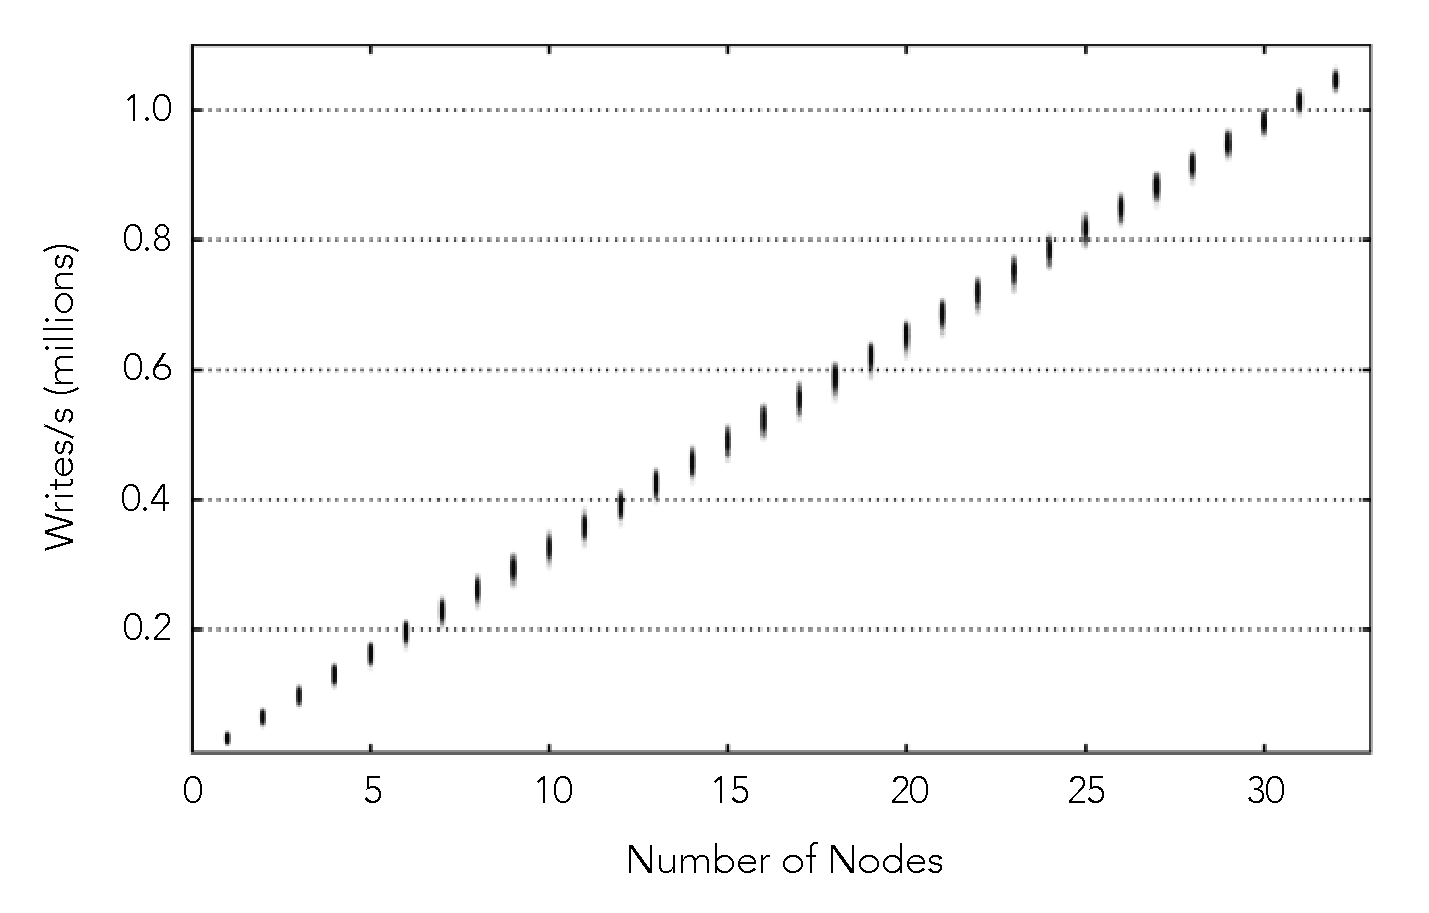
\includegraphics[width=0.7\textwidth]{figure_15.pdf}
  \caption{Write performance versus number of nodes. There is linear scaling in write performance with the number of nodes.}
  \label{fig:bigchain_writes_vs_nodes}
\end{figure}

Figure~\ref{fig:bigchain_writes_vs_nodes} shows data from the same experiment, except it shows how write throughput was affected by the number of nodes (rather than time).
The plot is both boring and exciting: it shows how write throughput increases linearly with the number of nodes.

\subsection{Other Experiments}
Appendix~\ref{appendix:benchmarks} contains descriptions and results of further experiments.